\providecommand{\main}{..}

\documentclass[/home/francois/latex/report/main.tex]{subfiles}

\begin{document}

\chapter{Background}
\label{chapter:background}

This chapter introduces the hardware setup, the mechanical models and the mathematical optimization framework that will be the core of the thesis:
%
% \section{Hardware setup}
% \label{section:hardware}
%
% Below are described the hardware equipement provided by the host organisation. It comprises the robotic arm, the \ac{FT} sensor attached to the last joint, the gripper tool and its \textit{suction cup}. A typical motion of the robot during \textit{pick-and-place} operation is described. Also, key physical behaviours of the system that influence the design of the mechanical models are highlighted.
%
% \subsection{Robotic manipulator}
%
% Two models of robotic 6 \ac{DoF} arms have been used throughout the project: UR10 and UR10e from \textsc{Universal Robot}\texttrademark. They are fairly similar since they can span an area of $1300 \si{\milli\meter}$ around them and can handle payload of $10 \si{\kilo\gram}$ –as sugested by the name. The particularity of UR10e is its built-in \ac{FT} sensor and faster communication ($500 \si{\hertz}$ by contrast with $125 \si{\hertz}$ of the UR10).
%
% \begin{figure}
%   \centering
%   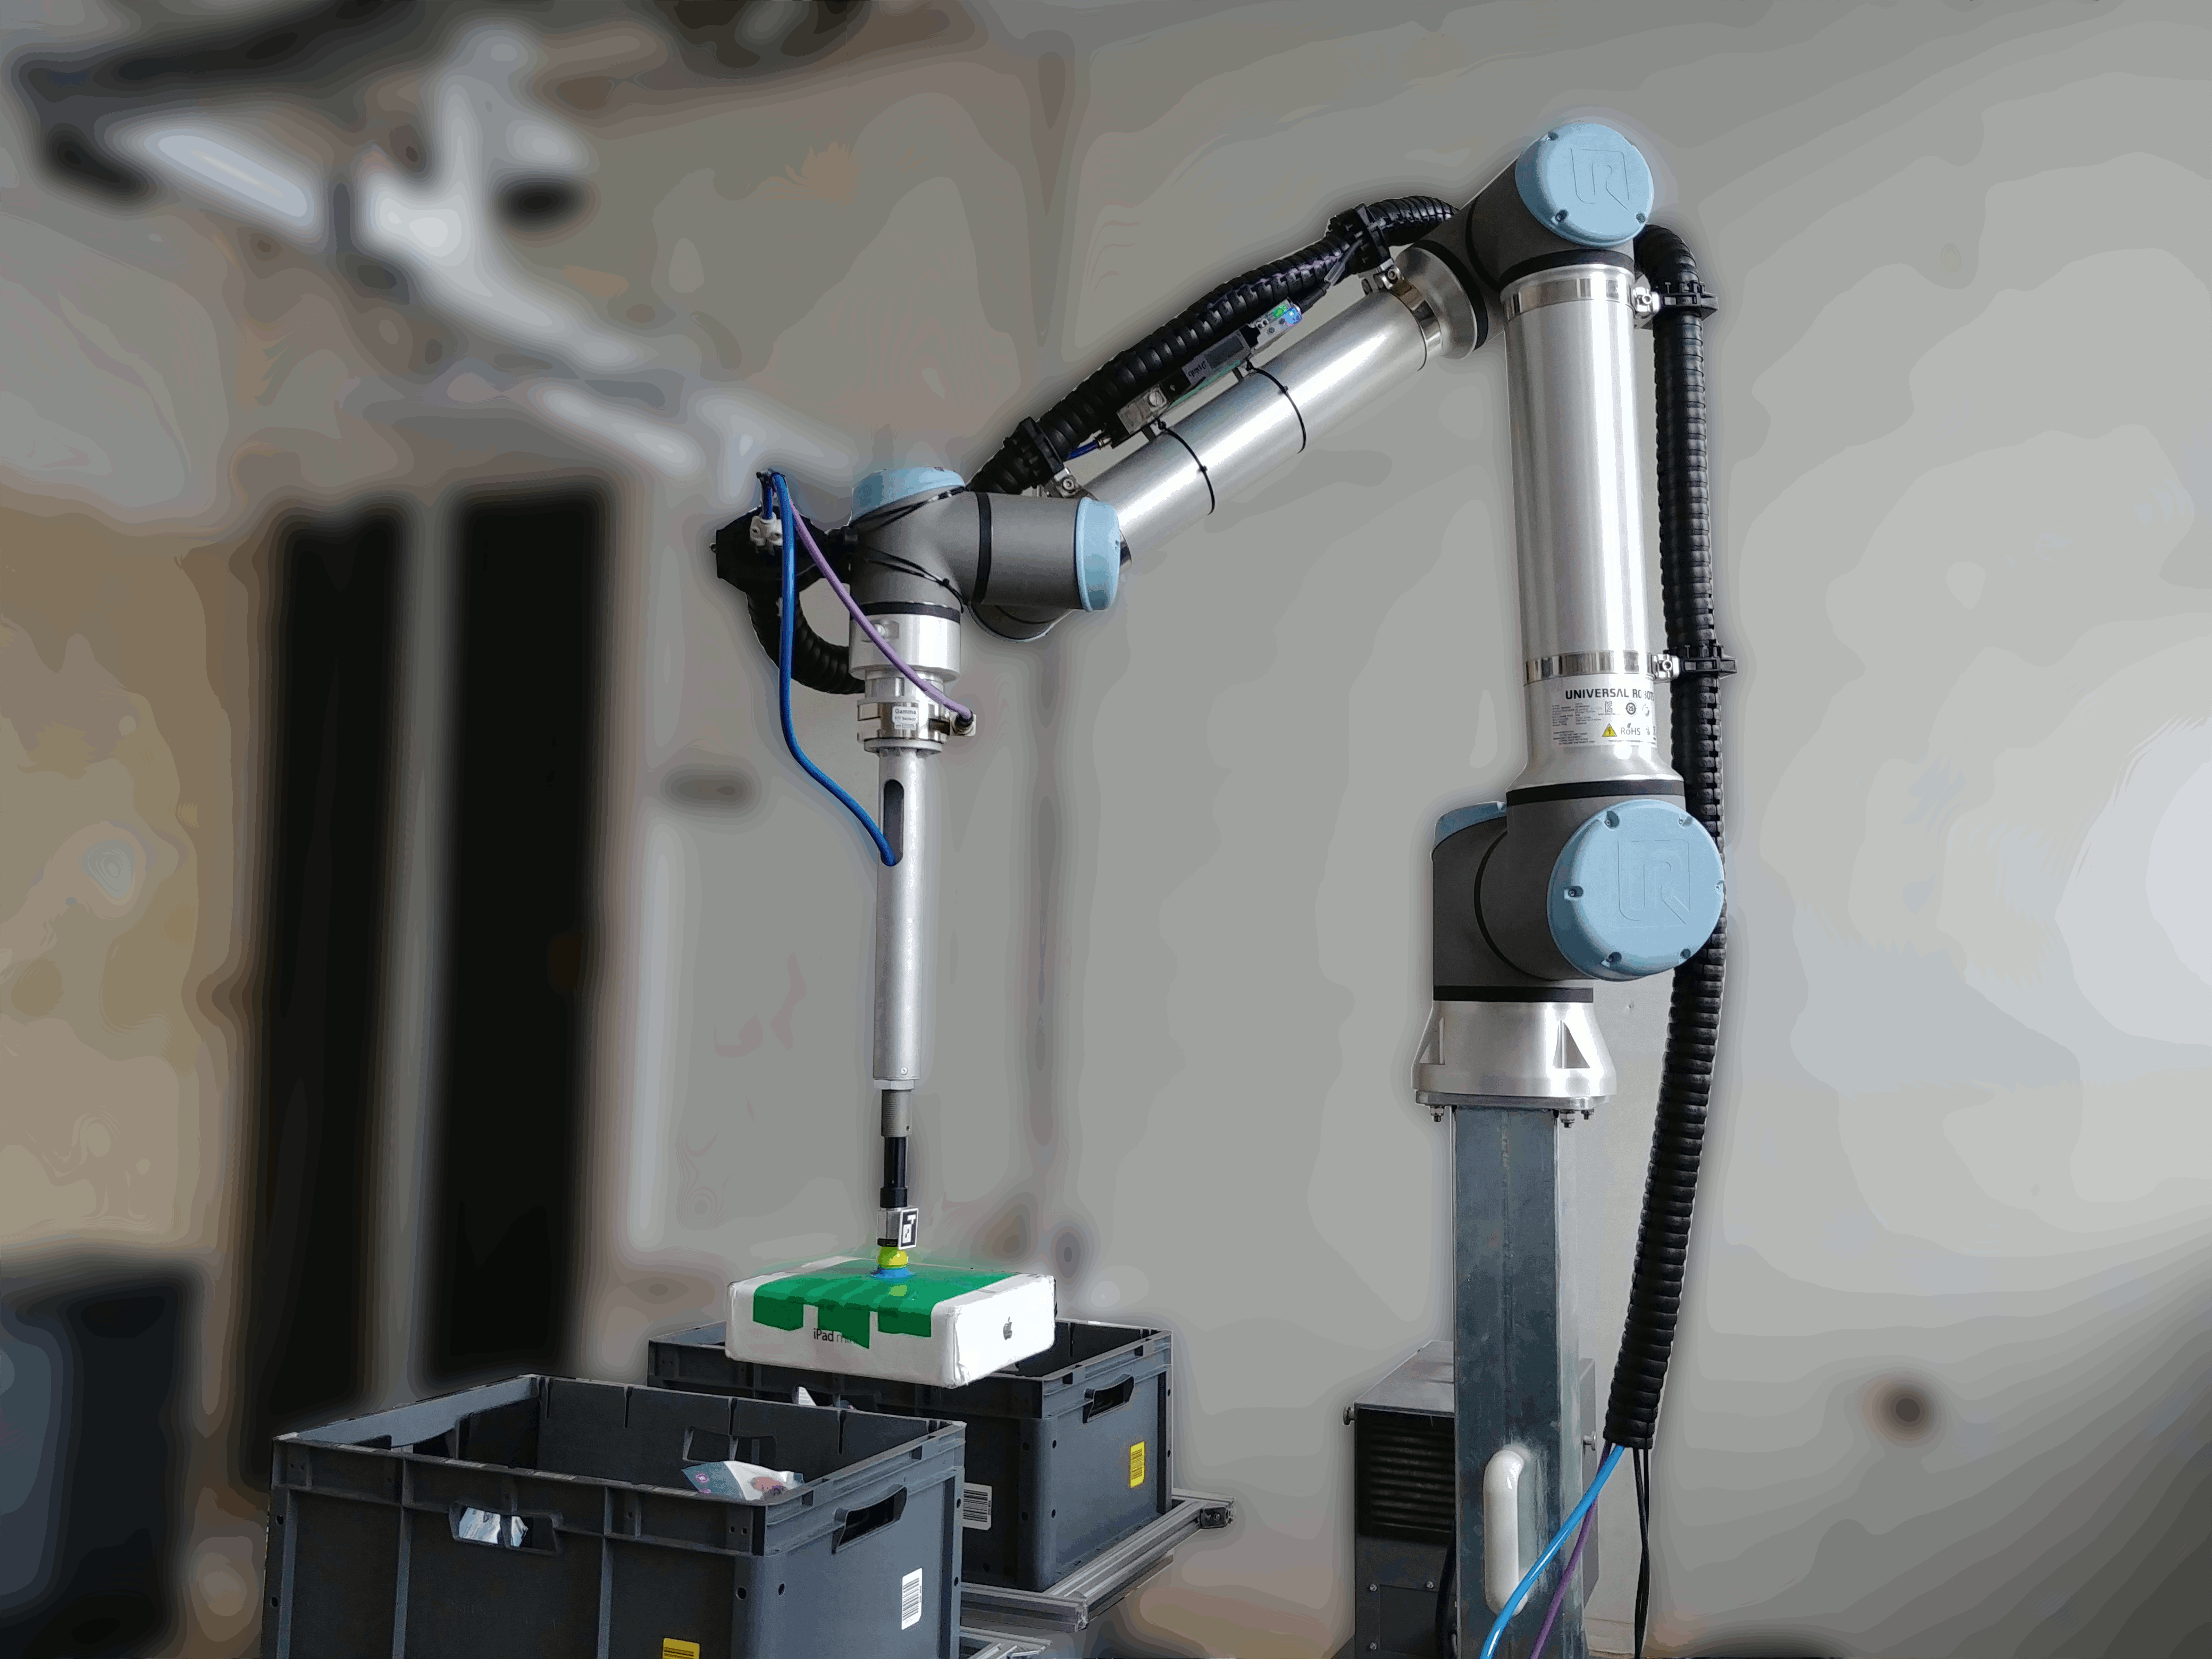
\includegraphics[scale=0.08]{\main/figures/picture_of_ur_indexed.png}
%   \caption{Robotic arm from \textsc{Universal Robot}\texttrademark \ grasping a box. Image from the author.}
%   \label{fig:background:albert}
% \end{figure}
%
% \subsection{\ac{FT} sensor}
%
% Two \ac{FT} sensors are used within the project. The built-in sensor of UR10e and the \textit{Gamma} \ac{FT} sensor from ATI\texttrademark. They are both mounted on the last joint of both robotic manipulators (see Figure \ref{fig:background:tool}). The ATI\texttrademark \ sensor is mostly used throughout the evaluation of the different approaches. Although its range of measurement is narrower than UR10e one, it has better resolution properties (see Table \ref{tab:background:ft-sensor}).
%
% \begin{table}[h!]
%   \begin{center}
%     \caption{Specifications of the built-in UR10e sensor and \textit{Gamma} sensor \cite{ati, ur10e}. }
%     \label{tab:background:ft-sensor}
%     \renewcommand{\arraystretch}{1.8} % Default value: 1
%     \begin{tabular}{l|c|c} % <-- Alignments: 1st column left, 2nd middle and 3rd right, with vertical lines in between
%       & \textbf{ATI Gamma} & \textbf{UR10e}\\
%       \hline
%       Range (force)  & $F_{x/y}: 32 \ \si{\newton}$ $F_z: 100 \ \si{\newton}$ & \underline{$100 \ \si{\newton}$} \\
%       \hline
%       Range (torque)  & $2.5 \ \si{\newton} \si{\meter}$ & \underline{$10 \ \si{\newton} \si{\meter}$} \\
%       \hline
%       Resolution (force)  & \underline{$F_{x/y}: 0.0062 \ \si{\newton}$ $F_z: 0.012 \ \si{\newton}$} & $2.0 \ \si{\newton}$ \\
%       \hline
%       Resolution (torque)  & \underline{$0.0005 \ \si{\newton} \si{\meter}$} & $0.02 \ \si{\newton} \si{\meter}$ \\
%       \hline
%     \end{tabular}
%   \end{center}
% \end{table}
%
% \subsection{End-effector}
%
% The end-effector of the robot fullfills the functions of grasping a wide range of items, measuring the force induced on the wrist, safely picking from diverse source totes, carts or conveyors. It consists of 4 basic elements (see Figure \ref{fig:background:tool}):
%
% \begin{itemize}
%   \item an ATI\texttrademark \ sensor which is screwed on the wrist of the robotic manipulator,
%   \item an extension tube to reach deep totes or carts,
%   \item a second cylinder inserted in the previous one with a safety-spring,
%   \item a vacuum suction cup linked to the hydraulic supply.
% \end{itemize}
%
% \begin{figure}
%   \centering
%   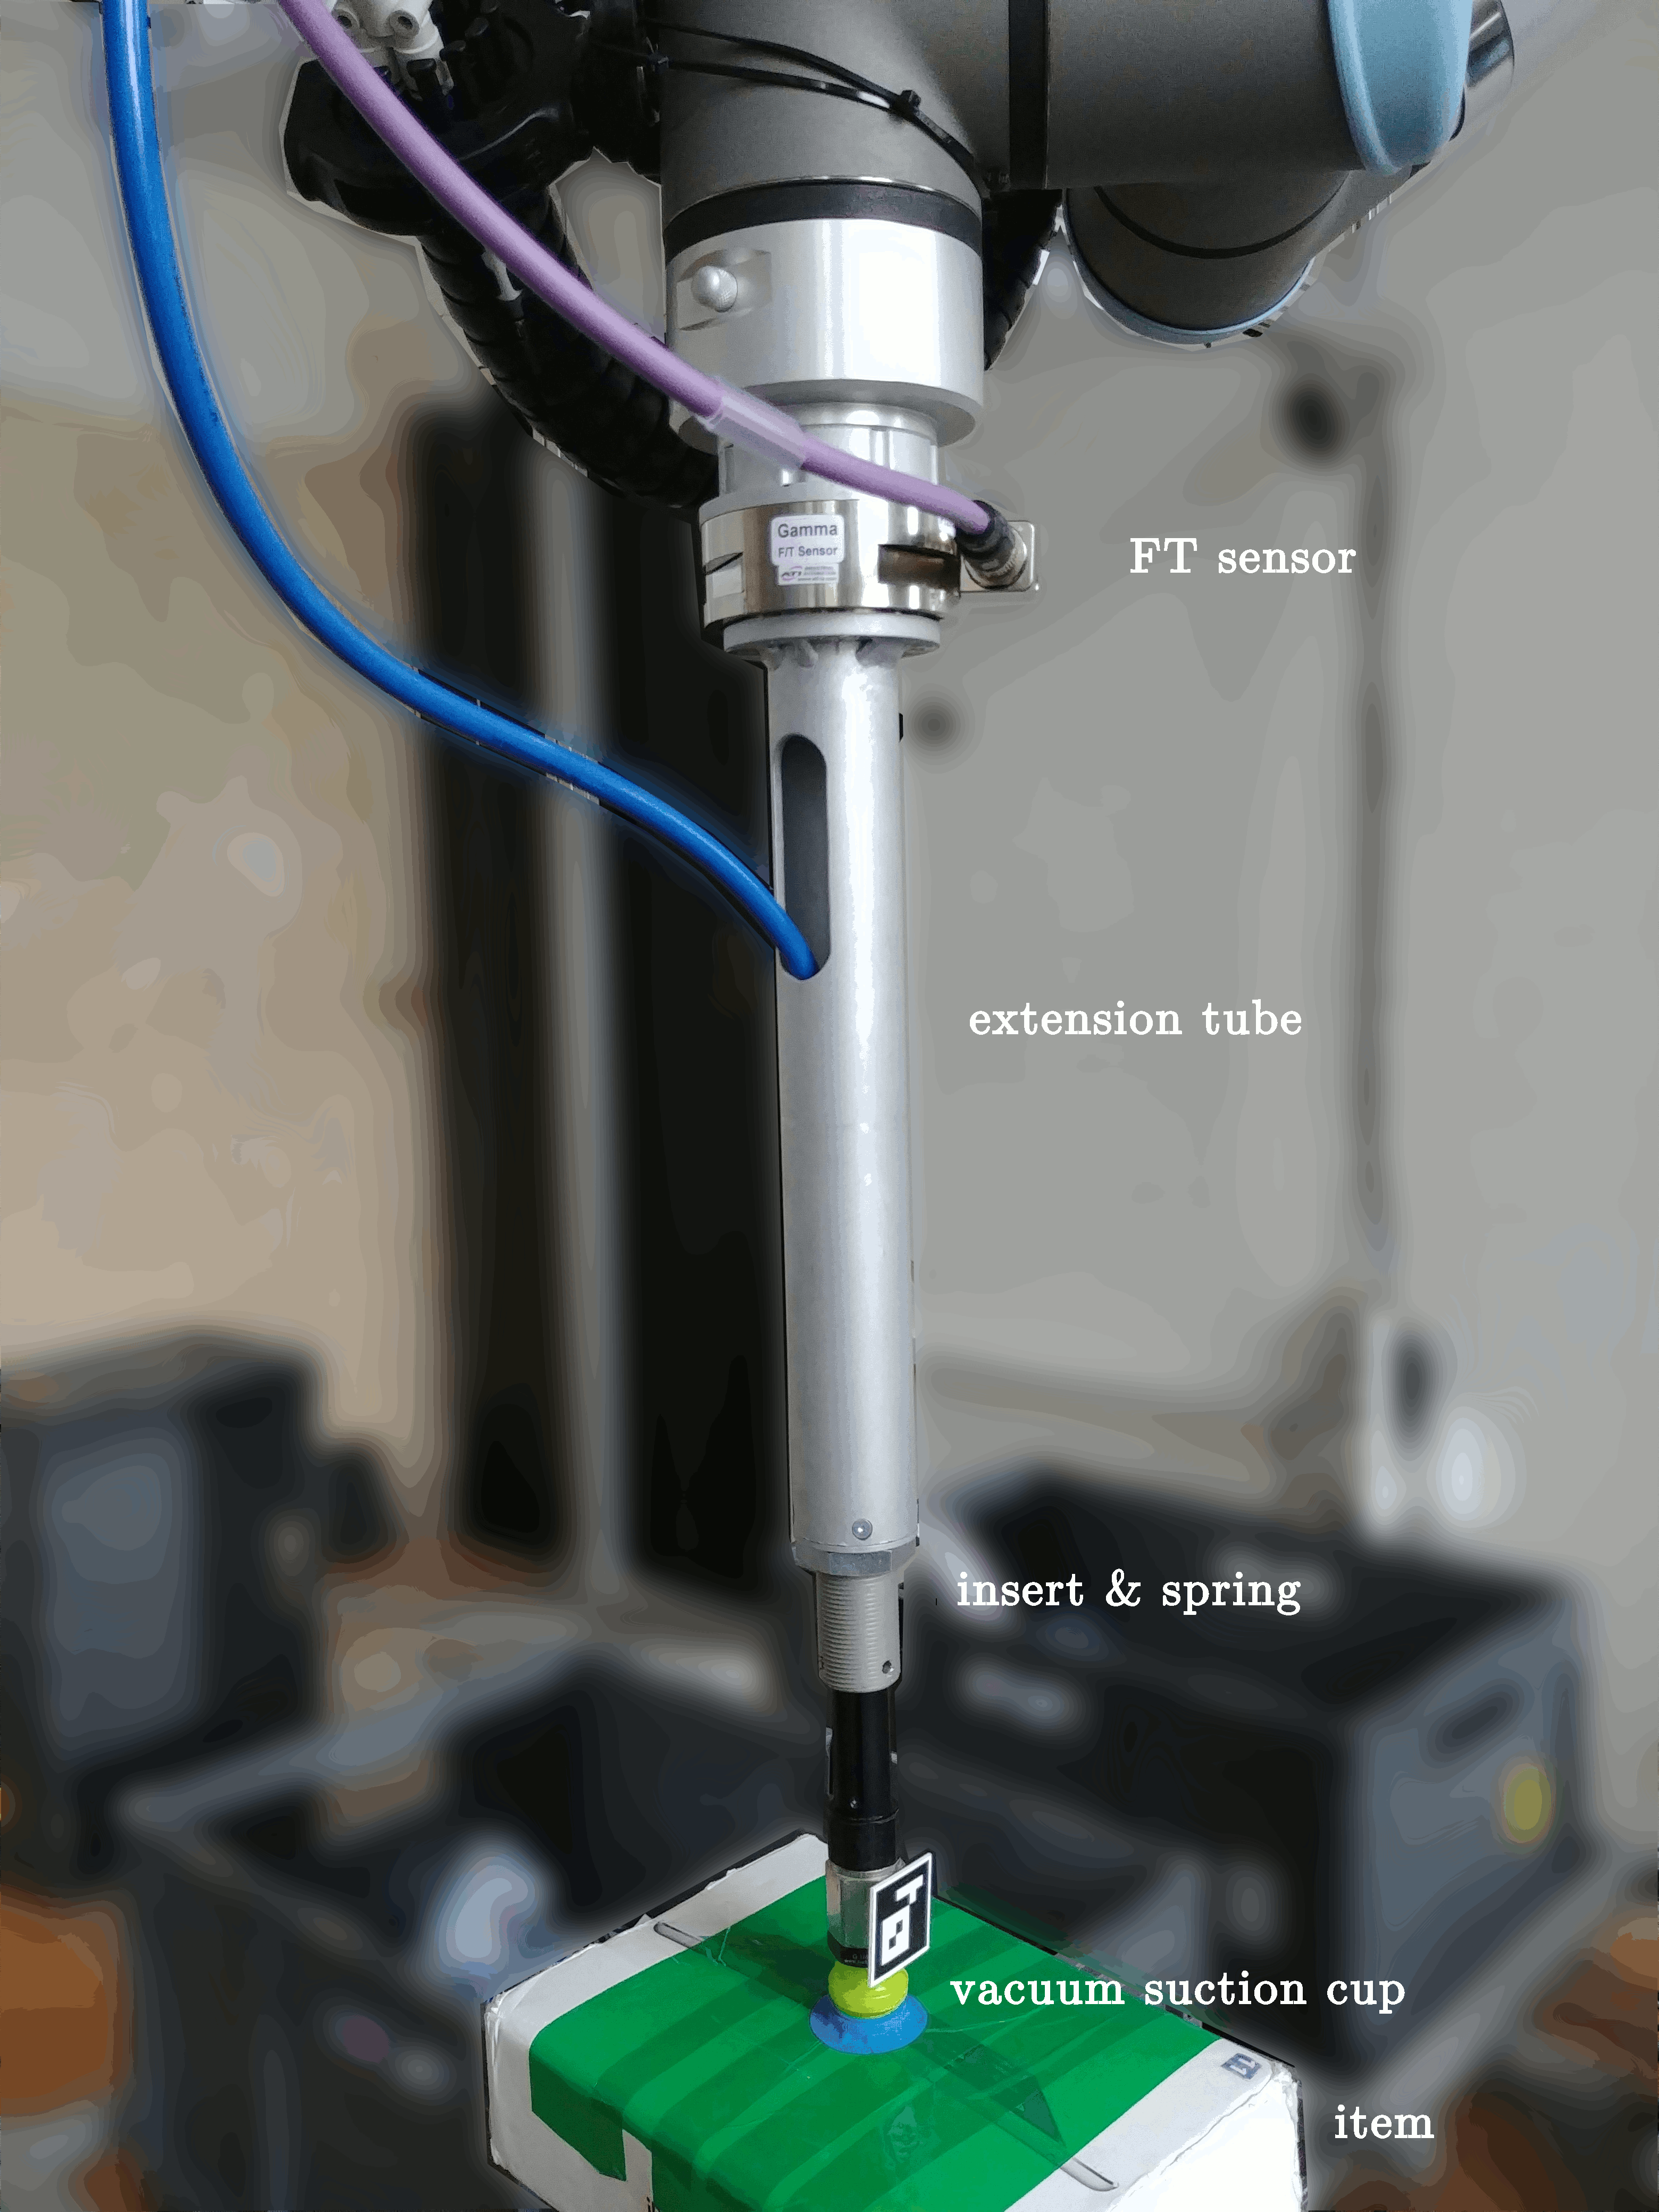
\includegraphics[scale=0.08]{\main/figures/picture_of_tool_indexed.png}
%   \caption{Tool mount on the robotic manipulator. Image from the author.}
%   \label{fig:background:tool}
% \end{figure}
%
% A suction cup with a springy extension is mounted on the tool. It allows a very simple integration logic and a versatile ability to grasp items (see Figure \ref{fig:background:suction}). The sealing lip provide a good grip on a large range of object textures.
%
% \begin{figure}
% \centering
% \begin{subfigure}{0.49\textwidth}
% \centering
% 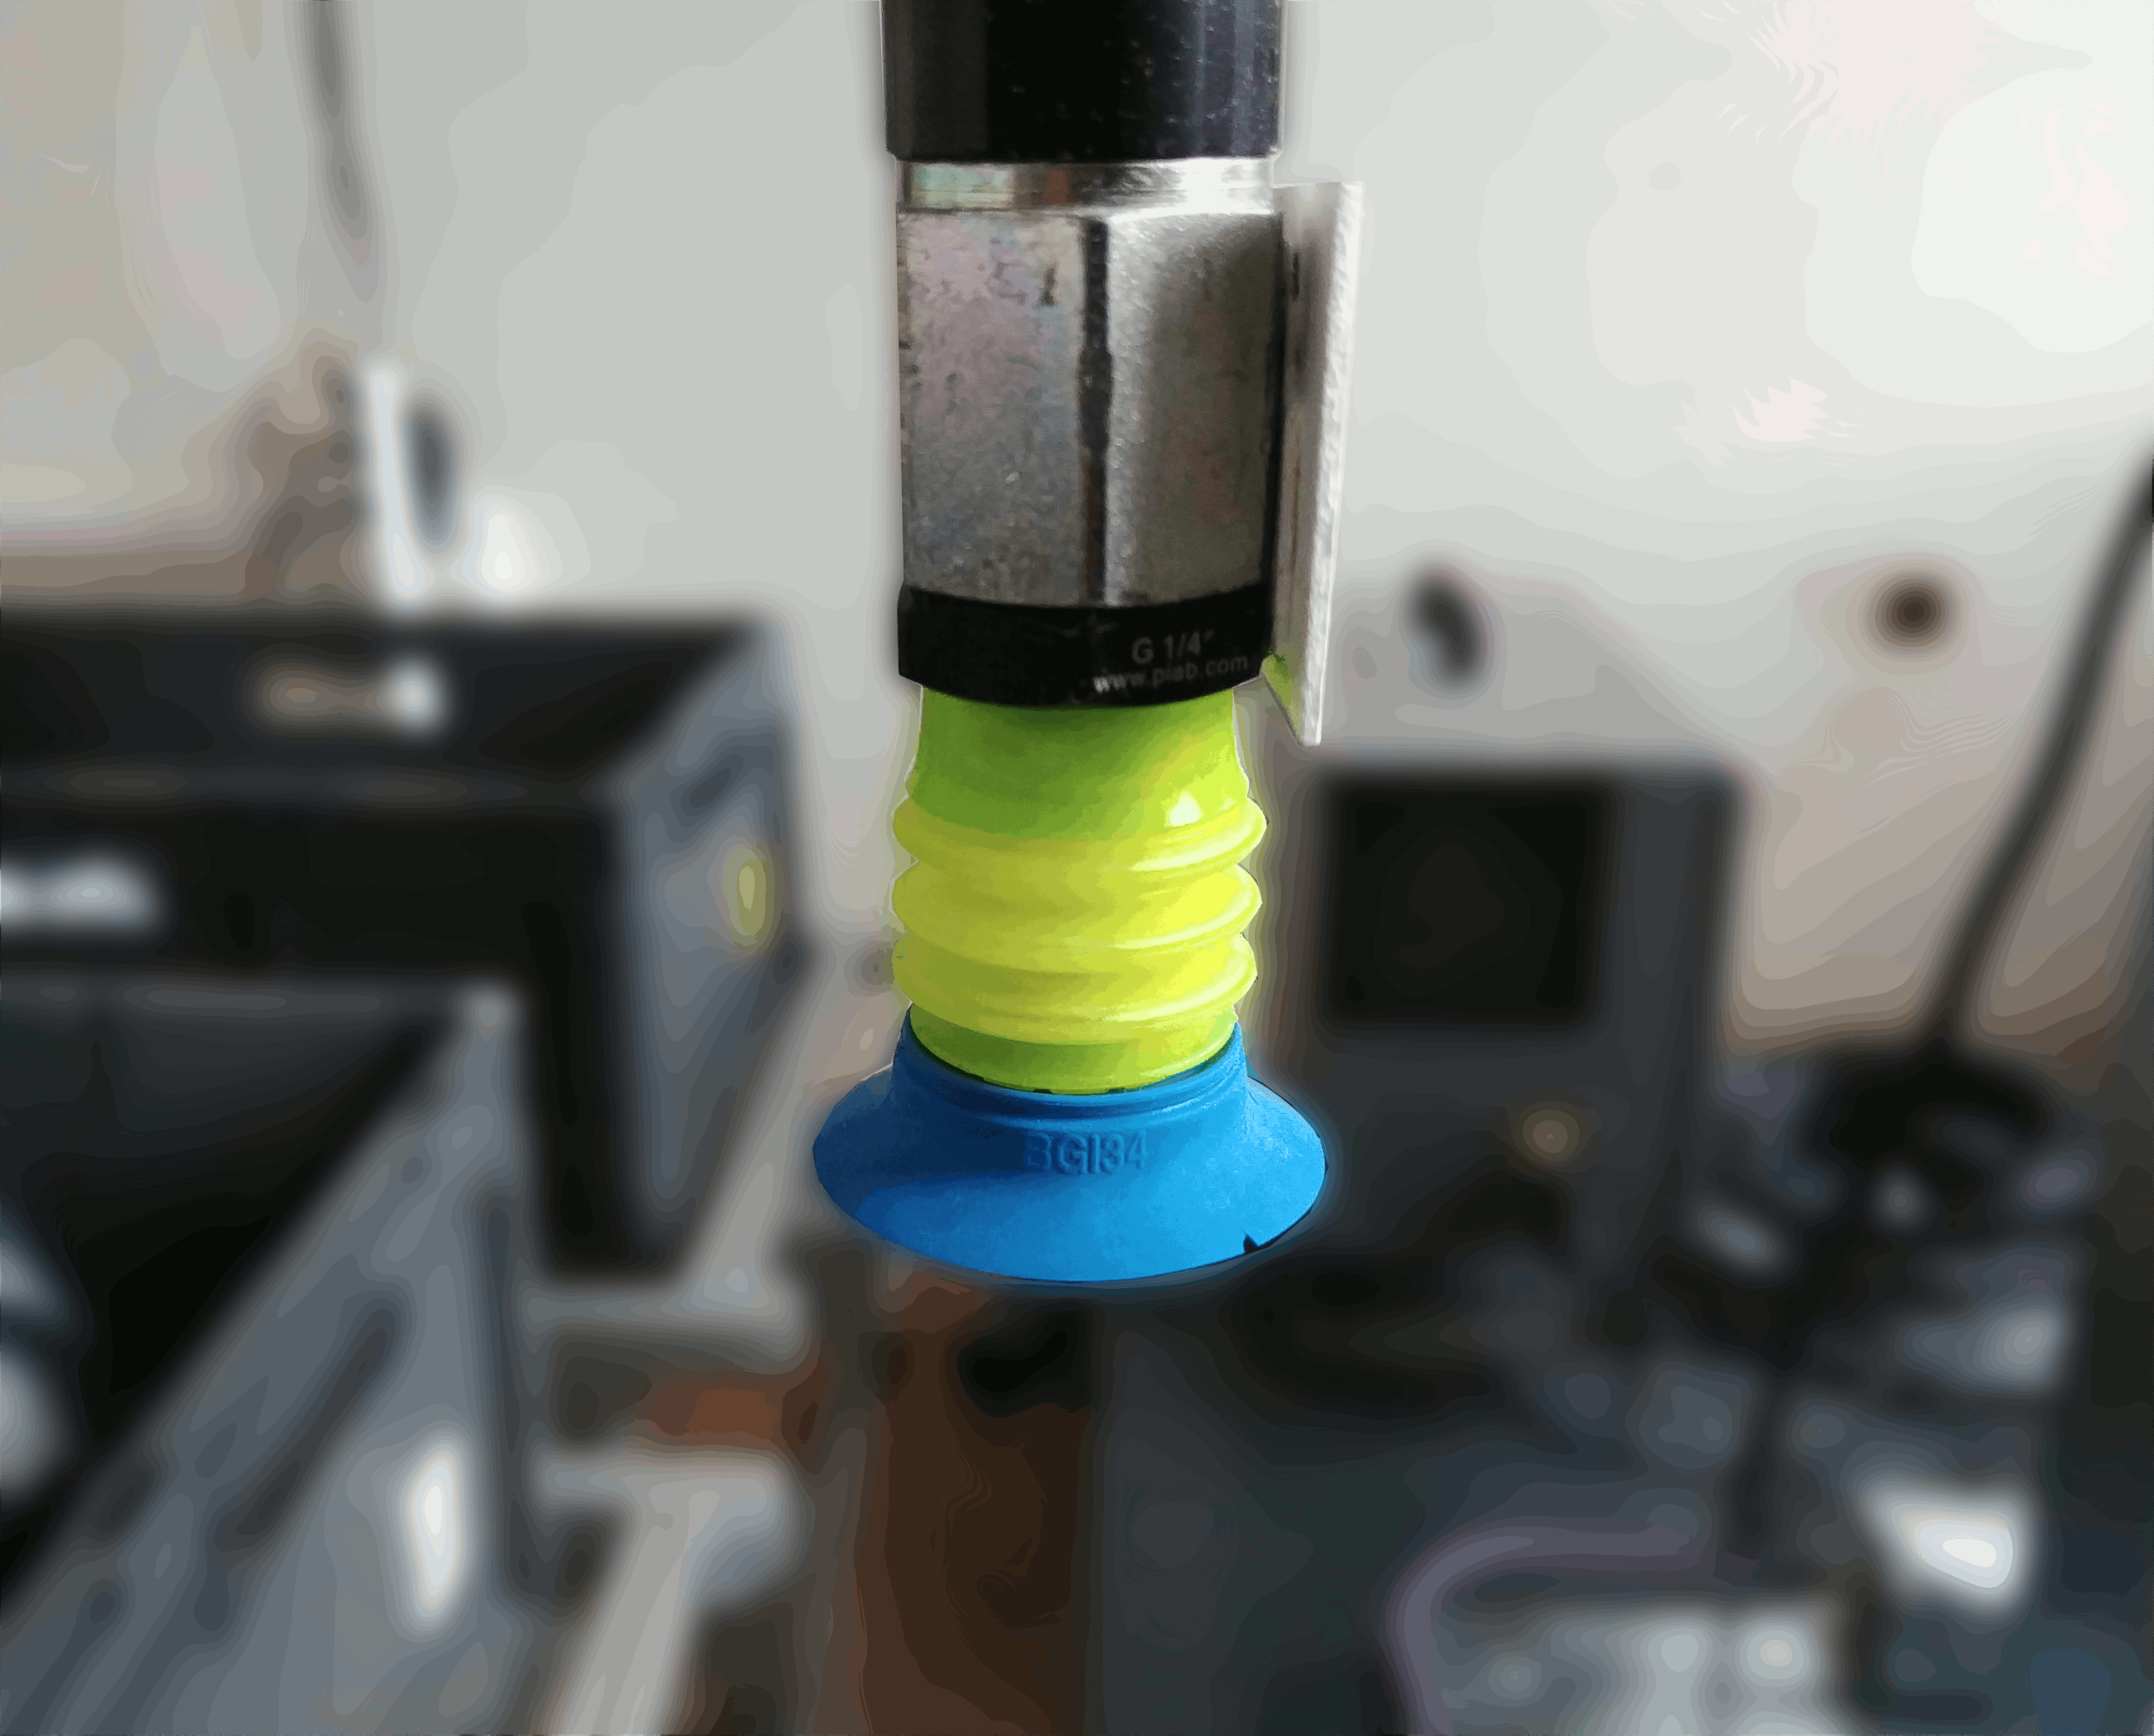
\includegraphics[scale=0.05]{\main/figures/suction_unloaded_indexed.png}
% \caption{Unloaded}
% \label{fig:background:suction-unloaded}
% \end{subfigure}
% \begin{subfigure}{0.49\textwidth}
% \centering
% 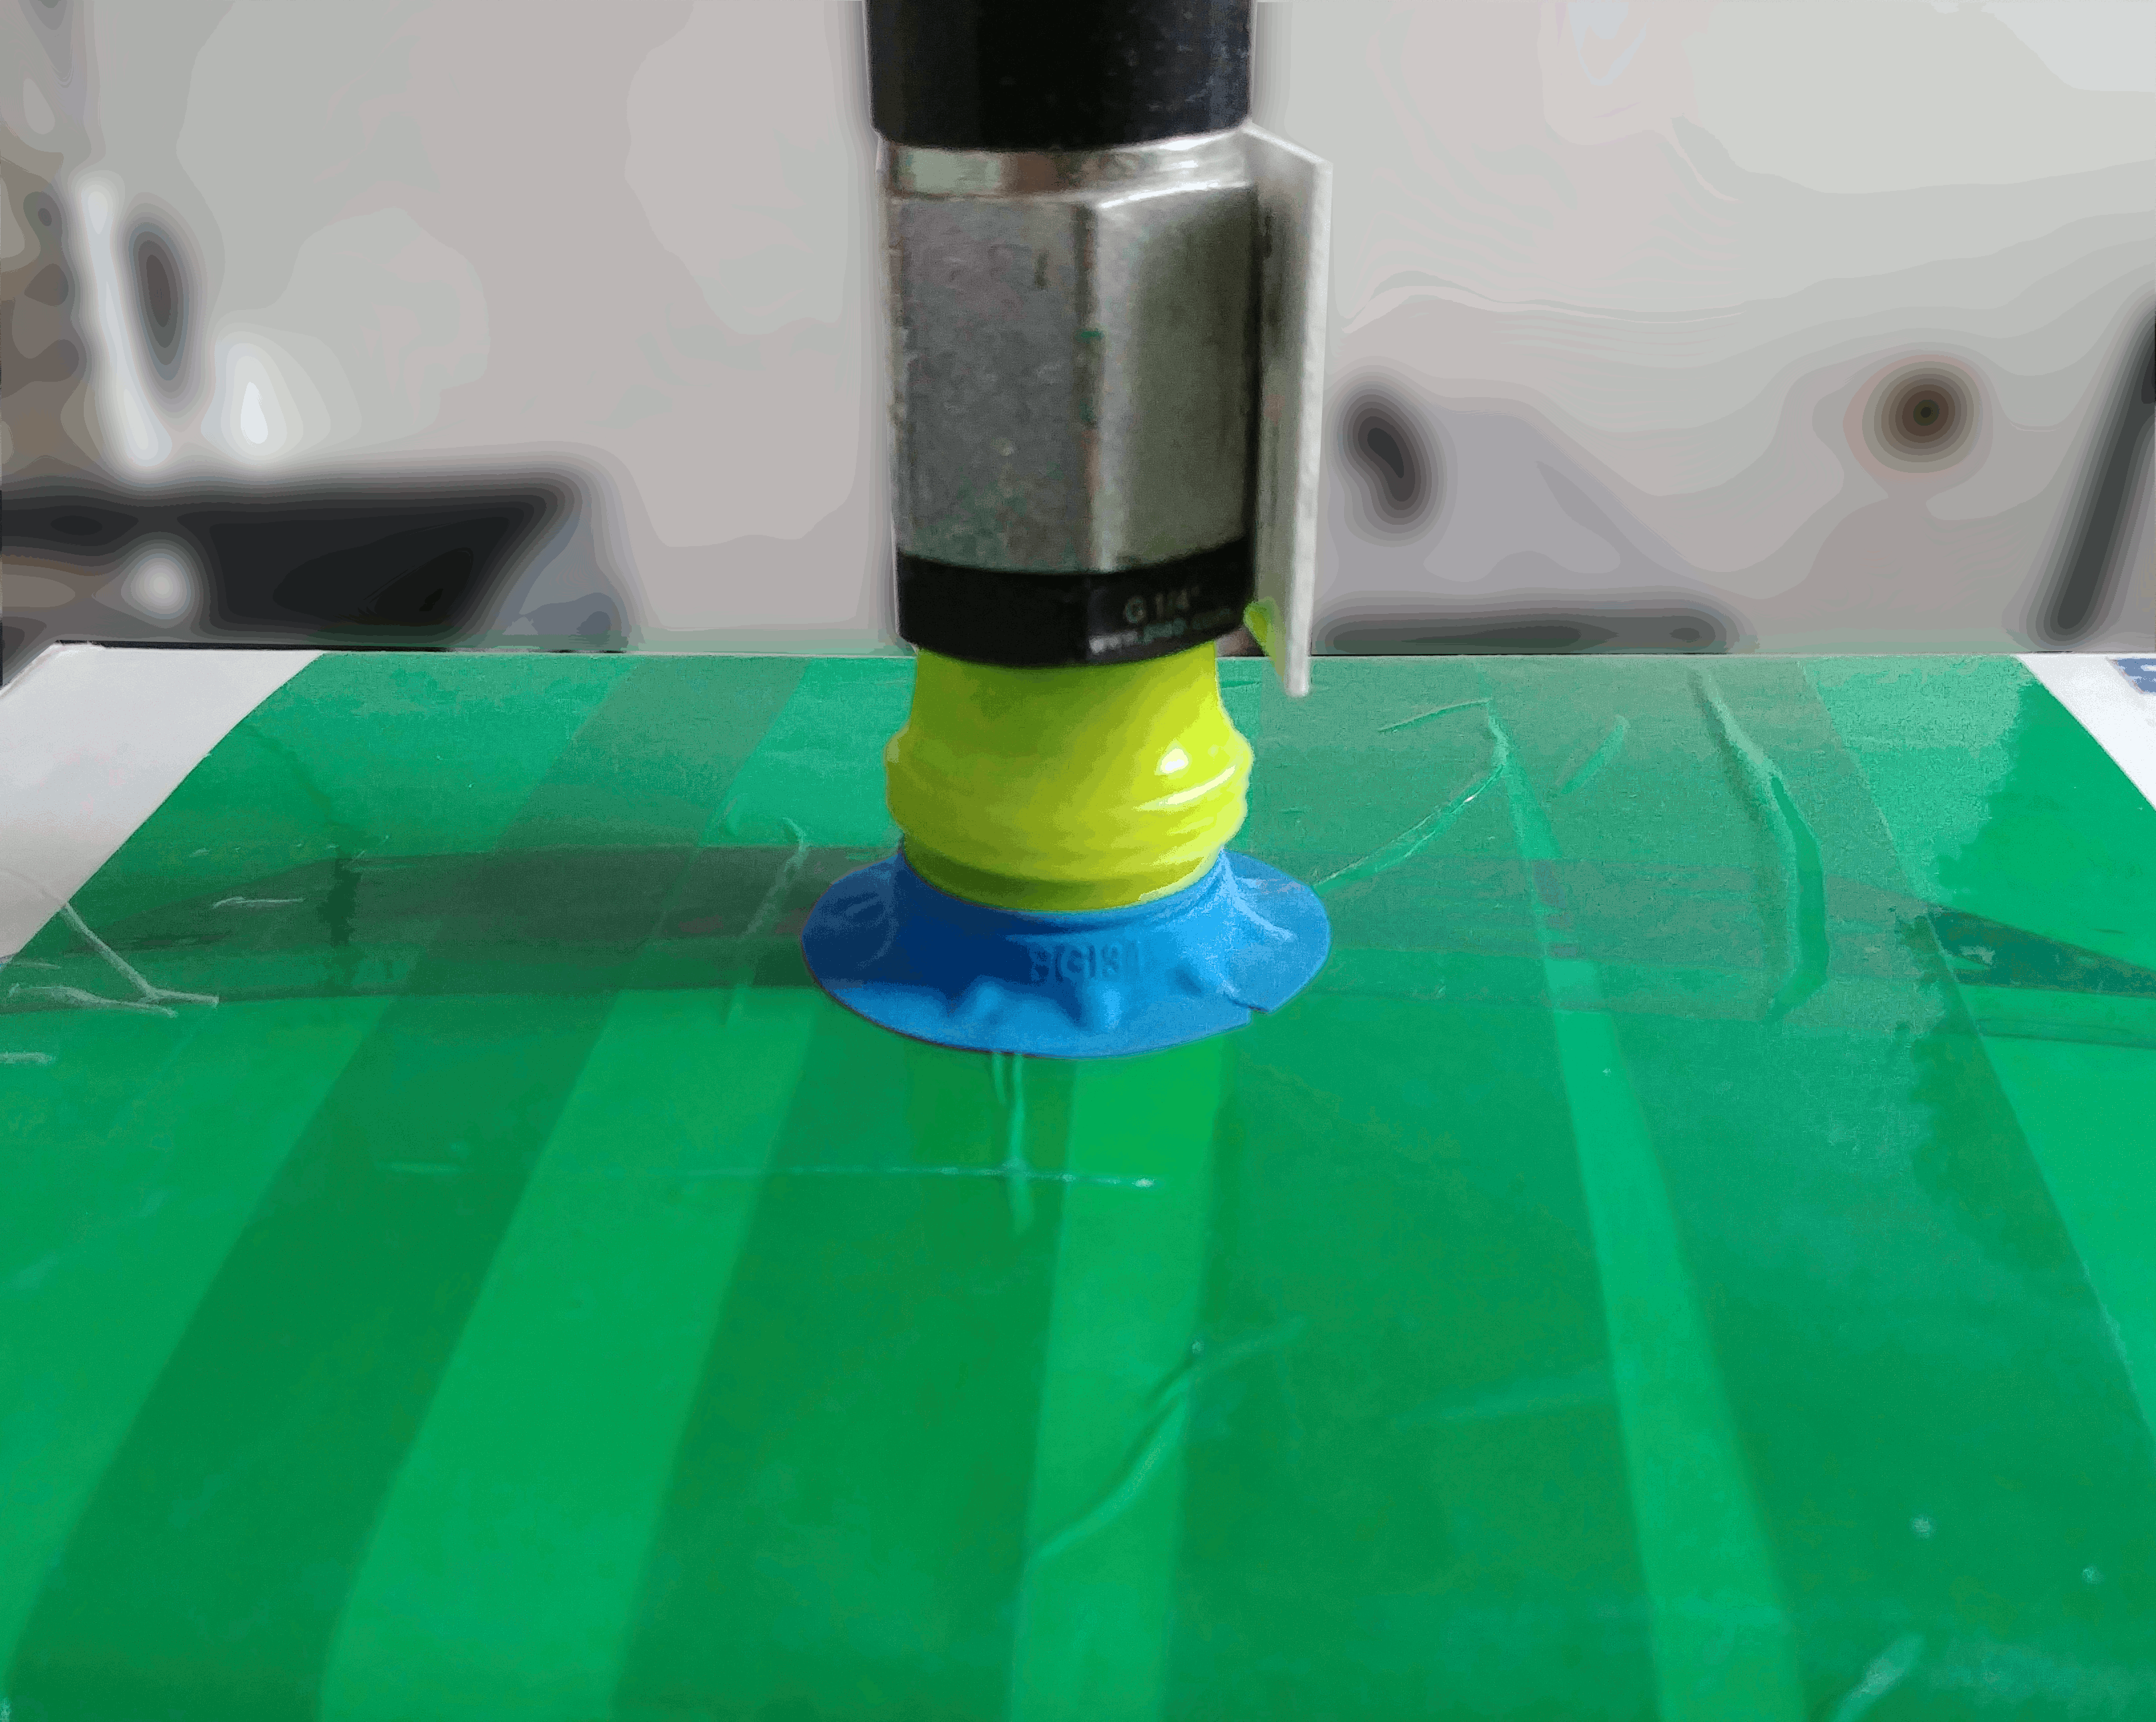
\includegraphics[scale=0.06]{\main/figures/suction_loaded_indexed.png}
% \caption{Loaded}
% \label{fig:background:suction-loaded}
% \end{subfigure}
% \caption{Vaccum suction cup gripper. Images from the author.}
% \label{fig:background:suction}
% \end{figure}
%
% \subsection{Characteristics of a typical \textit{pick-and-place} motion}
% \label{background:motion}
%
% In the context of \textit{pick-and-place} tasks, a robotic manipulator is meant to
% take an item from a given initial pose to a final pose \cite{Angeles2006}. This type of operation is exploited in tasks like loading and unloading of conveyor belts, totes, carts. In the use case of the project, trajectories have a blending trapezoidal shape. They are optimized for high production cadence and grasping failure avoidance (see Figure \ref{fig:background:tote_cycle}).
%
% \begin{figure}
%   \centering
%   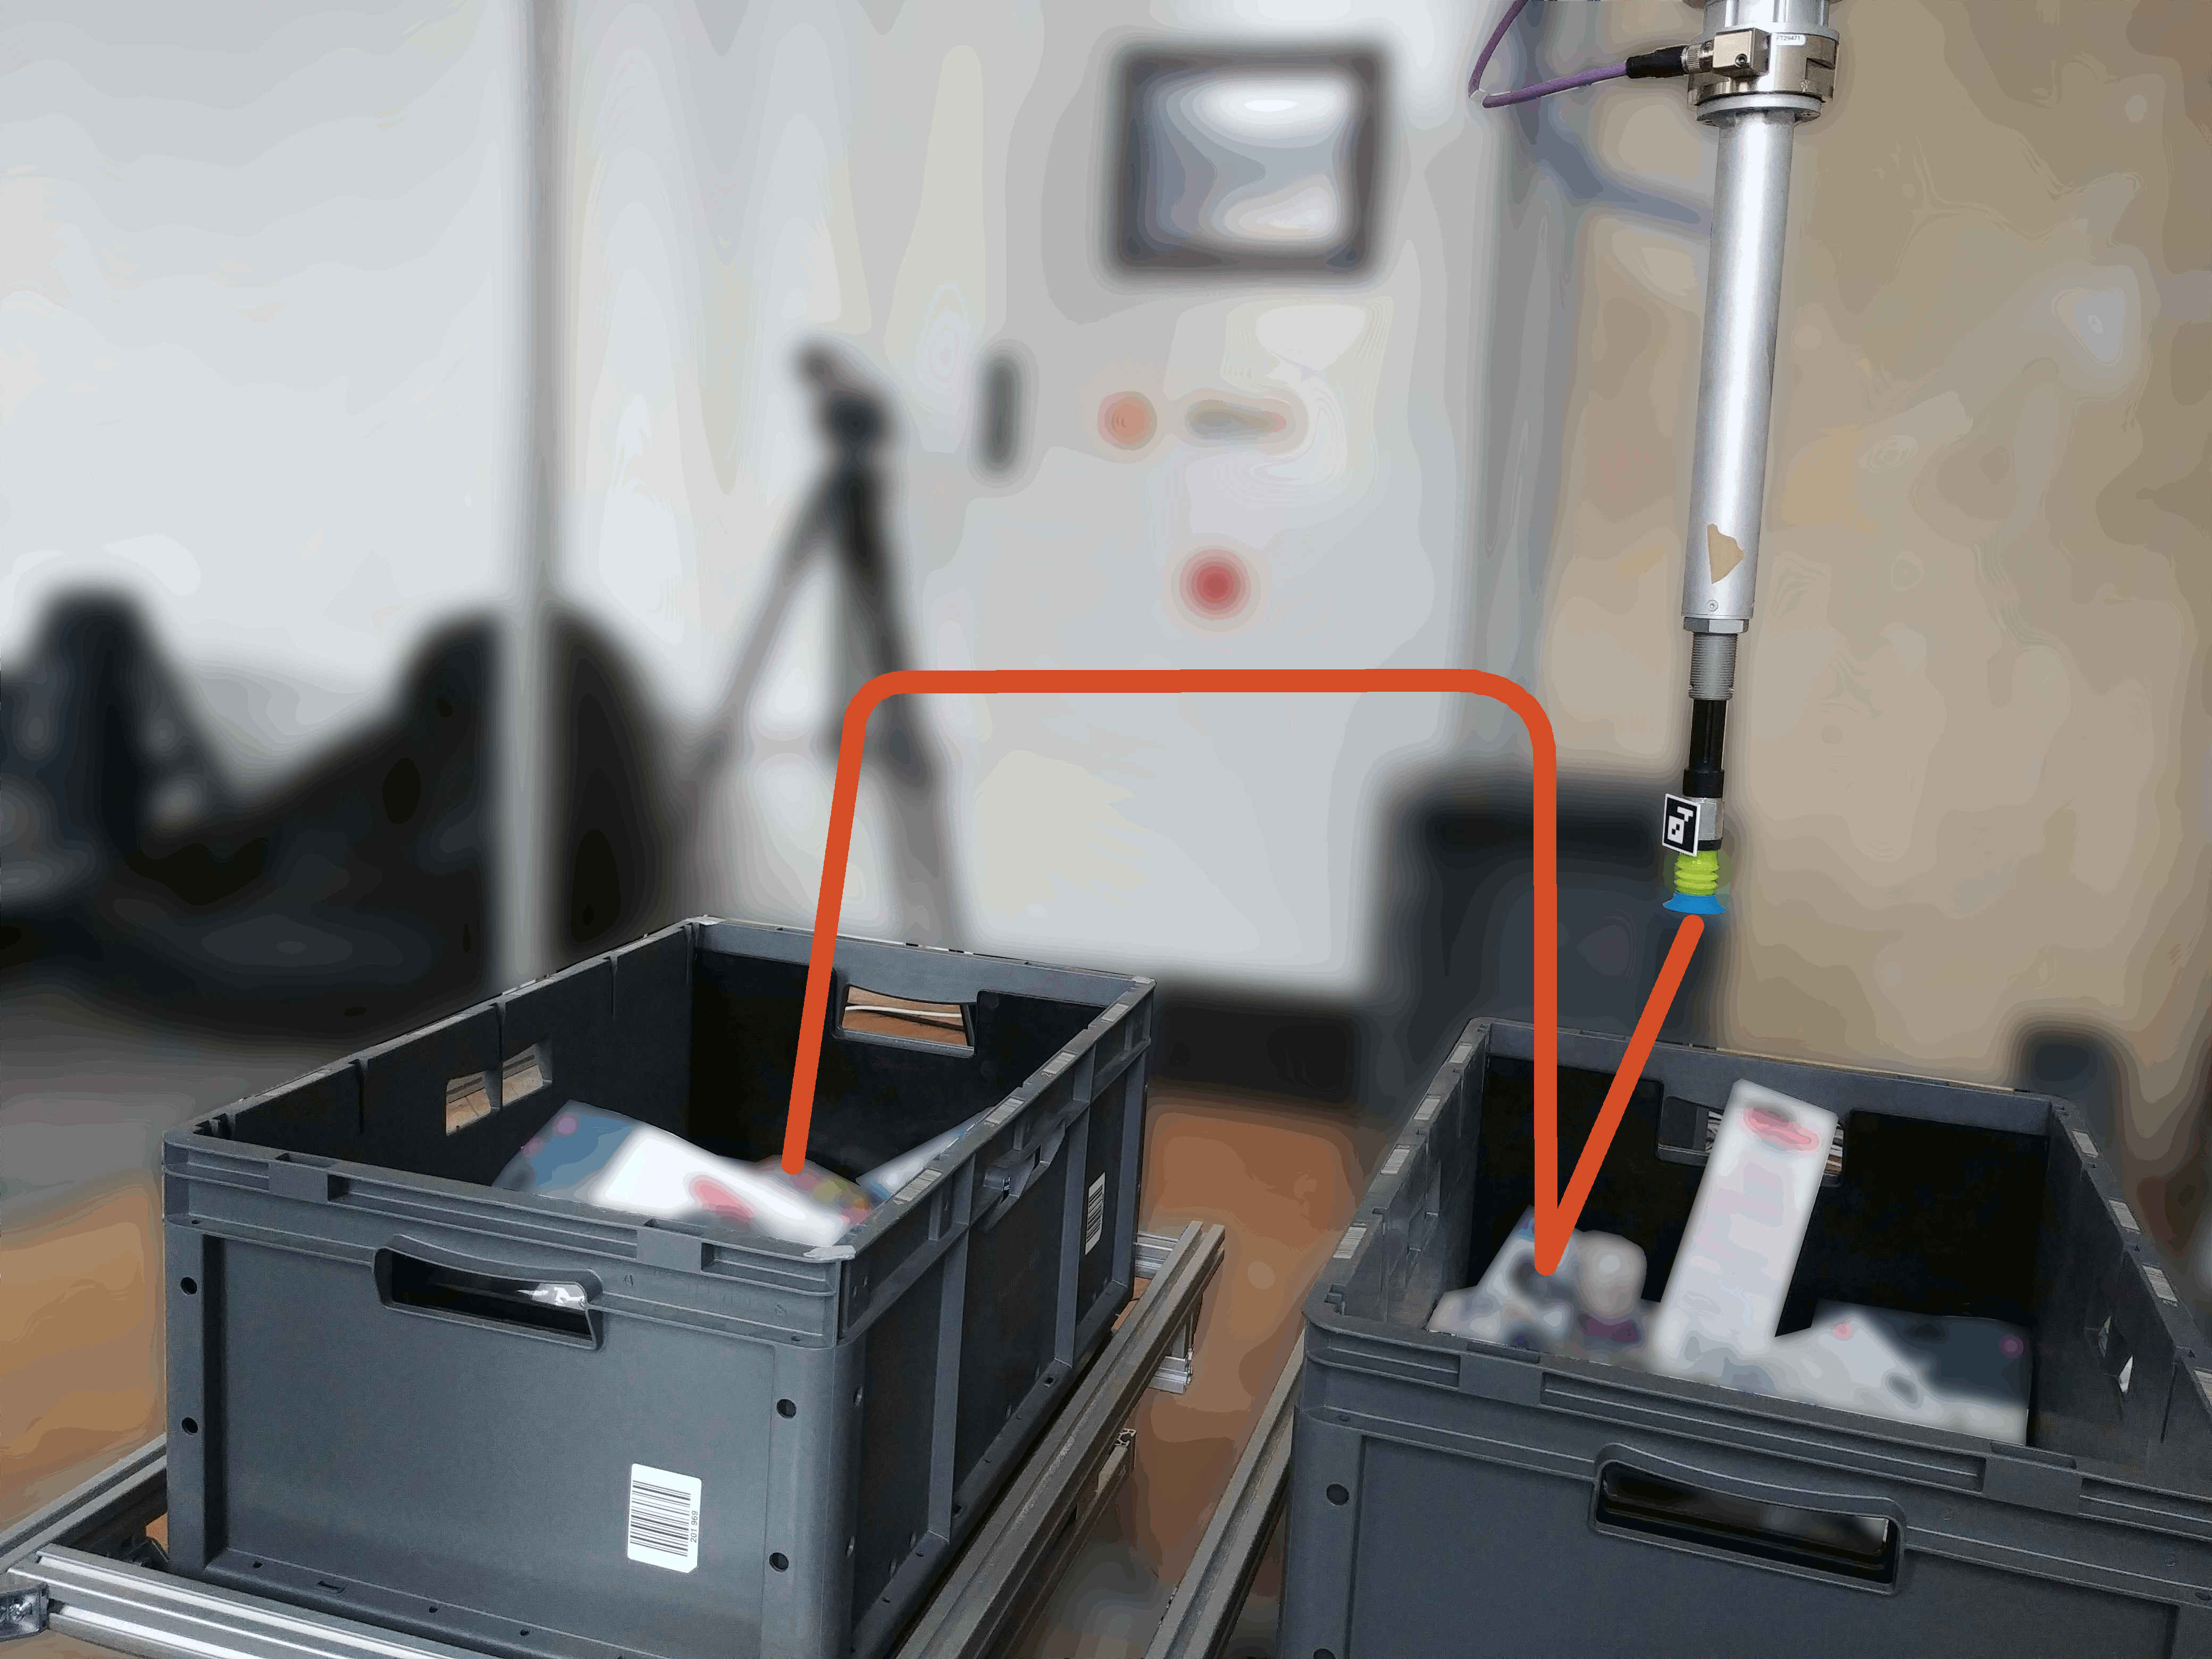
\includegraphics[scale=0.08]{\main/figures/tote_cycle_indexed.png}
%   \caption{Trajectory of the \ac{TCP} during a \textit{pick-and-place} cycle. Image from the author.}
%   \label{fig:background:tote_cycle}
% \end{figure}
%
% The drawback of using a suction cup for grasping is that the mechanical link between the tool and the item is not rigid. Heavy items and objects with large dimension are very likely to oscillate during the motion. In logistic warehouses, robots often handles object over half a kilo and longer dimension over $0.3 \si{\meter}$. Observations show that the angle between the tool and the item may vary significantly (up to $10 \si{\degree}$). Wobbling has a knock-on effect on \ac{FT} measurement. While there should not be any oscillations of the torque in a rigid model (for more detail, please refer to Section \ref{section:mechanical-models}), significant variations can be seen in actual measurement (see Figure \ref{fig:results:torque_}).
%
% When it comes to physically model the system, different level of details can be take into account. The first approach is to considered a rigid link between the tool and the item and a second approach is to fit an appropriate mechanical model considering the \ac{DoF} and the damped harmonic oscillator theory.

\section{Mechanical models}
\label{section:mechanical-models}

A lot of effort have been put into estimating the dynamic parameters of each rigid body link of robotic manipulators during the late century spent. An \textit{et al.} \cite{An1985} have developped a method to estimate the mass, the location of the center of mass and the moment of inertia of every link of a robotic arm. The method uses the joint torques and the calculation of the kinematics of the manipulator while moving. This work provide a sound method to derive the dynamic equations. Liu \textit{et al.} enhanced this approach in 1998 \cite{Liu1998} by using a proper filtering method for velocity that avoid difficult-to-measure acceleration measurements. Both teams were working with robotic manipulators mounted \textit{on} a six-axis \ac{FT} sensor.

More compact \ac{FT} sensors have been developped and more complex use cases needed to quantify robot interactions with its environment. Therefore, it is possible to mount \ac{FT} sensors on the last wrist and benefit from a more sensible measurement. A several research project have taken advantage of that and have developped payload inertial parameters estimation methods \cite{Kubus2008, Kubus2007, Kubus2014, Farsoni2018}. These methods similarly derive \textsc{Newton-Euler} equations in order to isolate a set of 10 inertial parameters: mass, center of mass and independant inertia tensor coeficients.

This section presents the rigid-assumptions mechanical model and a observation-based \ac{RMSD} two-bodies model.

\subsection{Rigid model of the \{tool + item\} system}

The equations exploited to estimate the inertial parameters of the \{tool + item\} body (mass $m$, coordinates of the center of mass $c$, and inertia matrix $I$) are derived from the basic laws of dynamics. The motion of a rigid body (\{tool + item\}) due to external forces and torques can be described based on the \textsc{Newton-Euler} equations.

The assumptions are as followed (illustrated in Figure \ref{fig:tikz:one_body}):

\begin{itemize}
 \item \ac{FT} sensor ($S$) measures the force $f$ and torque $\tau$ applied on the \{tool + item\} system,
 \item the \ac{TCP} ($A$) moves with a linear acceleration $a$, an angular acceleration $\alpha$ and an angular velocity $\omega$,
 \item the \{tool + item\} system is composed of the extension tube, spring, suction cup –of total mass $m_1$, center of mass $c_1$ and inertia matrix $I_1$– and the object –of mass $m_2$, center of mass $c_2$ and inertia matrix $I_2$,
 \item Centers of mass and inertia matrices are defined w.r.t.\ point $S$ such that $c = \overrightarrow{SG}$, $c_1 = \overrightarrow{SG_1}$ and $c_2 = \overrightarrow{SG_2}$.
\end{itemize}

\begin{figure}
\centering
   % \documentclass[tikz]{standalone}

% \usetikzlibrary{patterns}

\tikzset{cross/.style={cross out, draw=black, minimum size=2*(#1-\pgflinewidth), inner sep=0pt, outer sep=0pt},
%default radius will be 1pt.
cross/.default={4pt}}


% \begin{document}
\begin{tikzpicture}[thick,>=latex,->]


\begin{scope}
\clip(-5,6) rectangle (5,-4);
% \draw[step=1cm,gray,very thin] (-5,6) grid (10,-5);

% \filldraw[white] (-4.3,4.3) rectangle (4.3,0);
% \draw[double distance=1.6mm] (0,0) -- (3,-3) node[midway,xshift=4mm,yshift=2mm]{$\ell$};
% \draw[->] (3,-3) -- (3,-4.5) node[below]{$m\cdot g$};
% \draw[->] (3,-3) -- (2.,-2.0) node[left,yshift=-3mm]{$F$};
% \draw[fill=white] (-.5,.25) -- (.5,.35) -- (1.2,0.2) -- (-1.2,-0.2) -- cycle;
% \draw[fill=white] (-.4,1) -- (-.7,.9) -- (-.3,.8) -- (-.7,.7) -- (-.3,.5) -- (-.7,.4) -- (-.5,.25) -- (.5,.35) --  (.7,.5) -- (.3,.6) -- (.7,.7) -- (.3,.8) -- (.7,.9) -- (.4,1) -- cycle;
\draw[fill=white] (-4, -3) -- (-4, 0) -- (4, 0) -- (4,-3) -- cycle;


% \draw[draw=black,fill=white] (0, 0) circle circle (.3cm);
% \draw[draw=black,fill=white] (3,-3) circle circle (.3cm);
\draw[->] (2.6,4.1) -- (4,4.1) node[above]{$\overrightarrow{y_0}$};
\draw[->] (2.6,4.1) -- (2.6,5.5) node[right]{$\overrightarrow{z_0}$};

% \draw[dash dot] (0,0) -- (2.55,0) node[below]{$\overrightarrow{y_0}$};
% \draw[dash dot] (0,0) -- (2.5, .42) node[above]{$\overrightarrow{y_2}$};
% \draw[thick] ([shift=(0:2cm)]0,0) arc (0:20:1cm);
% \node[] at (2.3, .2) {$\theta$};

\draw[pattern=north east lines] (-.4,5.5) rectangle (.4,0);

\node[right] at (.5,5.5) {$S(y_1, z_1)$};
\draw[fill=white] (-.1, 5.4) -- (.1, 5.6) -- cycle;
\draw[fill=white] (-.1, 5.6) -- (.1, 5.4) -- cycle;

\node[below right] at (0,0) {A};
\draw[fill=white] (-.1, -.1) -- (.1, .1) -- cycle;
\draw[fill=white] (-.1, .1) -- (.1, -.1) -- cycle;

\node[right] at (0.3,1.5) {$G$};
\draw[fill=white] (-.1, 1.4) -- (.1, 1.6) -- cycle;
\draw[fill=white] (-.1, 1.6) -- (.1, 1.4) -- cycle;

\node[right] at (.2,-1.5) {$G_2$};
\draw[fill=white] (-.1, -1.6) -- (.1, -1.4) -- cycle;
\draw[fill=white] (-.1, -1.4) -- (.1, -1.6) -- cycle;

\node[right] at (0.3,2.5) {$G_1$};
\draw[fill=white] (-.1, 2.4) -- (.1, 2.6) -- cycle;
\draw[fill=white] (-.1, 2.6) -- (.1, 2.4) -- cycle;

\node[rotate=0] at (-3,-0.5) {$m_2$, $I_{2,A}$};

\end{scope}

\end{tikzpicture}
% \end{document}
 %     without .tex extension
   % or use \input{mytikz}
   \caption{Rigid \{tool + item\} system.}
   \label{fig:tikz:one_body}
\end{figure}

\subsubsection{Formulation of the \textsc{Newton-Euler} equations}
\label{subsubsection:background_newton_equation}

Detailed derivation of the \textsc{Newton-Euler} equation is presented in the Appendix \ref{appendix:models}. The method followed is fairly similar to the one proposed in \cite{An1985} except that equations are directly determined with respect to point $S$, in the base link frame. This variation pave the way to the second model which is derivated in a similar fashion with respect to point $A$.

Eventually, the dynamics of the rigid body is described by the equations \ref{background:eq:rigid} (see in equations \ref{background:eq:rigid} in Appendix \ref{appendix:models}) also used in \cite{Kubus2008, Kubus2007, Kubus2014, Farsoni2018}. They are \textit{linear} w.r.t.\ to the unknown parameters.

\begin{equation}
 \label{background:eq:rigid}
 \left \{
 \begin{array}{l l}
  f =    & m (a - g) + \omega \times (\omega \times m c) + \alpha \times m c \\
  \tau = & m c \times (a - g)
  + I_{S} \ast \alpha + \omega \times (I_{S} \ast \omega)
 \end{array}
 \right.
\end{equation}

where $I_S = I_S^T =
\begin{pmatrix}
 I_{xx} & I_{xy} & I_{xz} \\
 I_{xy} & I_{yy} & I_{yz} \\
 I_{xz} & I_{yz} & I_{zz}
\end{pmatrix}
$.

The equation \ref{background:eq:rigid} is exploited to compose the matrix equation \ref{background:eq:inertia_estimation} (see Appendix \ref{appendix:rigid:inertia_estimation} for detailed expression). This equation allows to isolate the 10 inertial parameters to be estimated. It can be easily adapted for least-squares-based estimation methods.

\begin{equation}
  \label{background:eq:inertia_estimation}
 \begin{pmatrix}
  f    \\
  \tau
 \end{pmatrix}
 = A(a, \alpha, \omega, g) \varphi
\end{equation}

where $\varphi = (m, m c_x, m c_y, m c_z, I_{xx}, I_{xy}, I_{xz}, I_{yy}, I_{yz}, I_{zz}) {}^T$ contains the 10 independant inertial parameters.

\subsection{\ac{RMSD} model of the \{tool + item\} system}

As mentioned in section \ref{background:motion}, the elasticity of the suction cup generate oscillation of the item w.r.t.\ tool that are not take into account by the one-rigid-body model. In fact, the object rotates about the $x_0$-axis the $y_0$-axis. There is no translation motion w.r.t.\ the tool and no rotation about the $z_0$-axis. Therefore, the mechanical link between the item and the tool can be identified as a \ac{UJ} –as known as \textsc{Cardan} joint (see Figure \ref{fig:background:cardan}). With this mechanical only, the tool can transfer forces, and torque about the lengthwise axis of the sensor but no torque about the transversal axes.

\begin{figure}
  \centering
  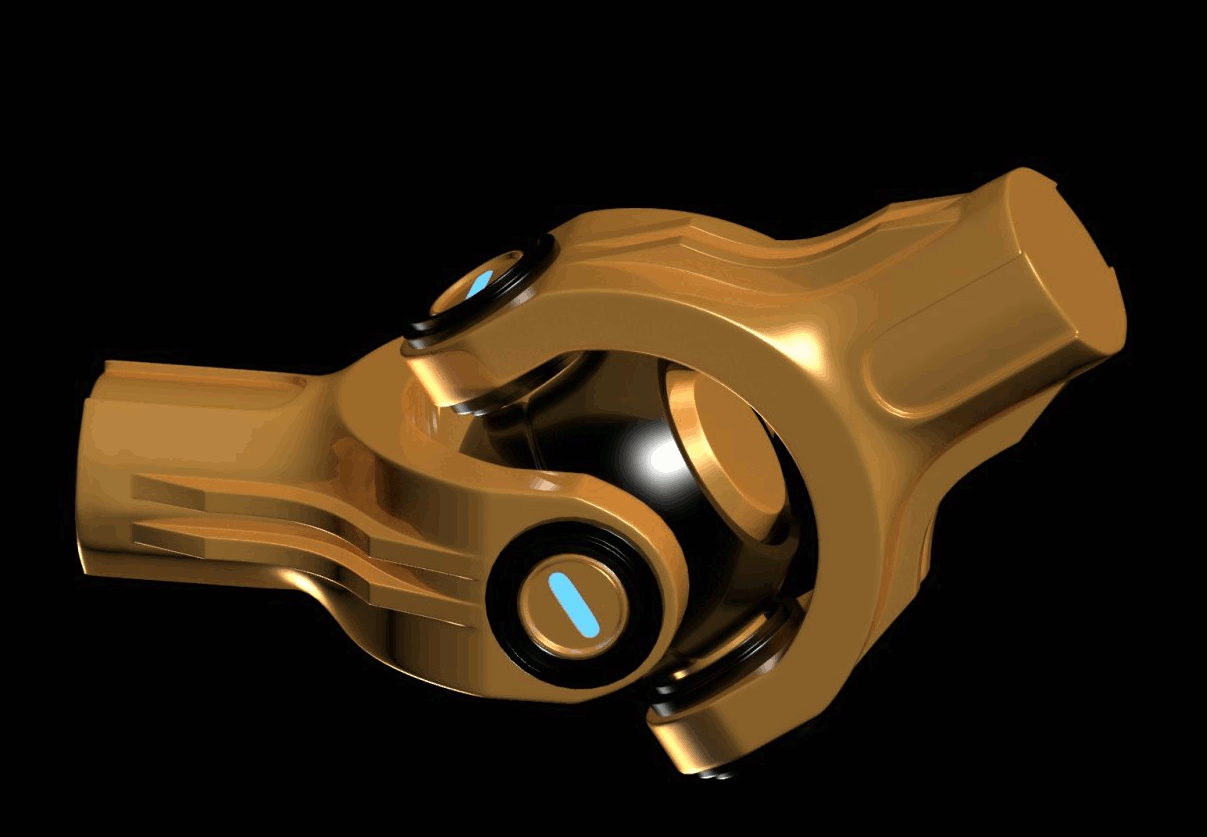
\includegraphics[scale=0.3]{\main/figures/cardan_joint_indexed.png}
  \caption{3D model of a 2 \ac{DoF} \ac{UJ}. Image from \cite{3dexport2020}.}
  \label{fig:background:cardan}
\end{figure}

One can notice that the combination of the two bodies behaves as a 2 \ac{DoF} harmonic pendulum. Thus, the torque transmitted by the tool \{1\} to the item \{2\} about the $x$-axis –or $y$-axis– is modeled by $T_{1/2, x} = k_x \theta_{1/2, x} + \lambda_x \dot{\theta}_{1/2, x}$ with $k_x$ a spring constant,  $\lambda_x$ a damping coefficient and $\theta_{1/2, x}$ the orientation of the tool w.r.t.\ the item about the $x$-axis. In addition, the suction cup is symetrical by rotation about the lengthwise axis of the tool. For this reason, it is considered that $k_x = k_y = k$ and $\lambda_x = \lambda_y - \lambda$.

This said, the total mechanical action of on the item \{2\} by the tool \{1\} is as followed (see \ref{appendix:notation:wrench} for notation and Figue \ref{fig:tikz:two_bodies}):

{\centering
 $ \{ \mathcal{V}_{1/2} \}
 = \leftidx{_{A}}{
  \left \{ \begin{array}{c}
  \overrightarrow{F}_{1/2} \\
  N_{1/2} \overrightarrow{z_1} +  K \ast \overrightarrow{\Theta}_{1/2} + \Lambda \ast \overrightarrow{\Omega}_{1/2}
  \end{array} \right \}
  }{}
 $
 \par}

 with $\overrightarrow{\Theta}_{1/2}$ the orientation of \{1\} w.r.t.\ \{2\}, $\overrightarrow{\Omega}_{1/2}$ the angular speed of \{1\} w.r.t.\ \{2\} and $K = diag(k, k, 0)$ and $\Lambda = diag(\lambda, \lambda, 0)$.

 \begin{figure}
 \centering
    % \documentclass[tikz]{standalone}

% \usetikzlibrary{patterns}

\tikzset{cross/.style={cross out, draw=black, minimum size=2*(#1-\pgflinewidth), inner sep=0pt, outer sep=0pt},
%default radius will be 1pt.
cross/.default={4pt}}


% \begin{document}
\begin{tikzpicture}[thick,>=latex,->]


\begin{scope}
\clip(-5,6) rectangle (5,-4);
% \draw[step=1cm,gray,very thin] (-5,6) grid (10,-5);

% \filldraw[white] (-4.3,4.3) rectangle (4.3,0);
% \draw[double distance=1.6mm] (0,0) -- (3,-3) node[midway,xshift=4mm,yshift=2mm]{$\ell$};
% \draw[->] (3,-3) -- (3,-4.5) node[below]{$m\cdot g$};
% \draw[->] (3,-3) -- (2.,-2.0) node[left,yshift=-3mm]{$F$};
\draw[fill=white] (-.5,.25) -- (.5,.35) -- (1.2,0.2) -- (-1.2,-0.2) -- cycle;
\draw[fill=white] (-.4,1) -- (-.7,.9) -- (-.3,.8) -- (-.7,.7) -- (-.3,.5) -- (-.7,.4) -- (-.5,.25) -- (.5,.35) --  (.7,.5) -- (.3,.6) -- (.7,.7) -- (.3,.8) -- (.7,.9) -- (.4,1) -- cycle;
\draw[fill=white] (-3.5, -3.6) -- (-4,-.667) -- (4,.667) -- (4.5,-2.27) -- cycle;


% \draw[draw=black,fill=white] (0, 0) circle circle (.3cm);
% \draw[draw=black,fill=white] (3,-3) circle circle (.3cm);
\draw[->] (2.6,4.1) -- (4,4.1) node[above]{$\overrightarrow{y_0}$};
\draw[->] (2.6,4.1) -- (2.6,5.5) node[right]{$\overrightarrow{z_0}$};

\draw[->] (0.0,5.5) -- (-1.4,5.5) node[below]{$\overrightarrow{y_1}$};
\draw[->] (0.0,5.5) -- (0.0,4.1);
\node[left] at (-0.3,4.1) {$\overrightarrow{z_1}$};


\draw[dash dot] (0,0) -- (2.55,0) node[below]{$\overrightarrow{y_0}$};
\draw[dash dot] (0,0) -- (-2.5, -.42) node[above]{$\overrightarrow{y_2}$};
\draw[thick] ([shift=(0:2cm)]0,0) arc (0:20:1cm);
\node[] at (2.3, .2) {$\theta$};

\draw[pattern=north east lines] (-.4,5.5) rectangle (.4,1);

\node[right] at (.5,5.5) {$S(y_1, z_1)$};
\draw[fill=white] (-.1, 5.4) -- (.1, 5.6) -- cycle;
\draw[fill=white] (-.1, 5.6) -- (.1, 5.4) -- cycle;

\node[below right] at (0,0) {A};
\draw[fill=white] (-.1, -.1) -- (.1, .1) -- cycle;
\draw[fill=white] (-.1, .1) -- (.1, -.1) -- cycle;

\node[right] at (0.3,1.5) {$G$};
\draw[fill=white] (.0, 1.4) -- (.2, 1.6) -- cycle;
\draw[fill=white] (.0, 1.6) -- (.2, 1.4) -- cycle;

\node[right] at (0.25,-1.46) {$G_2$};
\draw[fill=white] (.15, -1.56) -- (.35,-1.36) -- cycle;
\draw[fill=white] (.15, -1.36) -- (.35, -1.56) -- cycle;

\node[right] at (0.3,2.5) {$G_1$};
\draw[fill=white] (-.1, 2.4) -- (.1, 2.6) -- cycle;
\draw[fill=white] (-.1, 2.6) -- (.1, 2.4) -- cycle;

\node[rotate=10] at (-3,-0.8) {$m$, $I_{2,A}$};

\end{scope}

\end{tikzpicture}
% \end{document}
 %     without .tex extension
    % or use \input{mytikz}
    \caption{\ac{RMSD} \{tool\} and \{item\} system.}
    \label{fig:tikz:two_bodies}
 \end{figure}

\subsection{Sensor offset}

\textit{TODO}

{\it
Strategies to manage the (unknown) sensor offset \cite{Kubus2007, Kubus2008}.
}

\section{Estimation Approaches}

\subsection{Least-Squares method}

\textit{TODO}

{\it
Brief presentation of the method in order to highlight the limit of the least-squares method.
}

\subsection{Recursive Total Least-Squares technique}

\textit{TODO}

{\it
Recursive Total Least-Squares considers error $E$ in the data matrix and error $e$ in the \ac{FT} vector \cite{Kubus2008}
.

\begin{equation}
 \begin{pmatrix}
  f    \\
  \tau
 \end{pmatrix} + e
 = (A + E) \varphi
\end{equation}
}

\end{document}
